\chapter{机器学习中的损失函数}

\begin{introduction}
  \item regression loss
  \item binary classification loss
  \item multi-class classification loss
  \end{introduction}

\section{回归问题的损失函数}

常见的回归问题的损失函数包括:
\begin{itemize}
  \item 平方损失函数 (square loss 或 l2-loss): $L(\hat{y}, y) = (\hat{y} - y)^2$
  \item 绝对值损失函数 (absolute loss 或者 l1-loss):$L(\hat{y}, y) = |\hat{y} - y|$
  \item Huber损失函数:当$|\hat{y} - y|\leq\delta$,$L(\hat{y}, y)$为$(\hat{y} - y)^2$;当$|\hat{y} - y|>\delta$,$L(\hat{y}, y)$为$|\hat{y} - y|$
\end{itemize}

平方损失函数 (square loss)在处理回归问题时最常见,且其具有光滑可导、凸性等优点。但平方损失函数的缺点在于,它对异常点 (outliers) 敏感。这里,敏感指的是由于平方损失函数的形式,异常点会最终“贡献”较大的损失值,从而导致模型在训练过程中过于受异常点的影响。我们可以以最大似然的角度解释平方损失函数:对于样本点$\bm{x}_i$,样本标签$y_i$的噪声$\epsilon^{(i)}$独立同分布,且服从于均值为0,标准差为$\delta$的高斯分布$\mathcal{N}(0,\delta)$。那么在整个训练集上的似然为:
\begin{equation}
  \begin{aligned}
    L(\bm{\theta}) &= \prod_{i=1}^{n}{p(y^{(i)}|\bm{x}^{(i)};\bm{\theta})}
  \end{aligned}
\end{equation}

绝对值损失函数 (absolute loss) 相对平方损失函数对异常点较不敏感。但该损失函数在$y=0$时不可导,且当$\hat{y}$非常接近$y$时,$|\frac{\partial L}{\partial \hat{y}}|=1$,导致优化过程中当参数接近极值点时可能发生震荡,此时的优化收敛性相较于使用平方损失函数时差。绝对值损失函数也可以从最大似然角度解释,只不过样本标签的噪声满足Laplace分布:

\begin{definition}[Laplace分布] \label{def:laplace} 
  一元维度上的Laplace分布密度函数为:
  \begin{equation}
    Lap(x|\mu, b) = \frac{1}{2b}\exp\left(-\frac{|x-u|}{b}\right)
  \end{equation}
  基于此定义的Laplace分布的均值为$\mu$,方差为$2b^2$。
\end{definition}

Huber损失函数可以看作平方损失函数和绝对值损失函数的结合,对异常点没有平方损失函数那样敏感,损失函数光滑可导,并且在靠近极值点时具有平方损失函数的性质。

\begin{figure}[htbp]
  \centering
  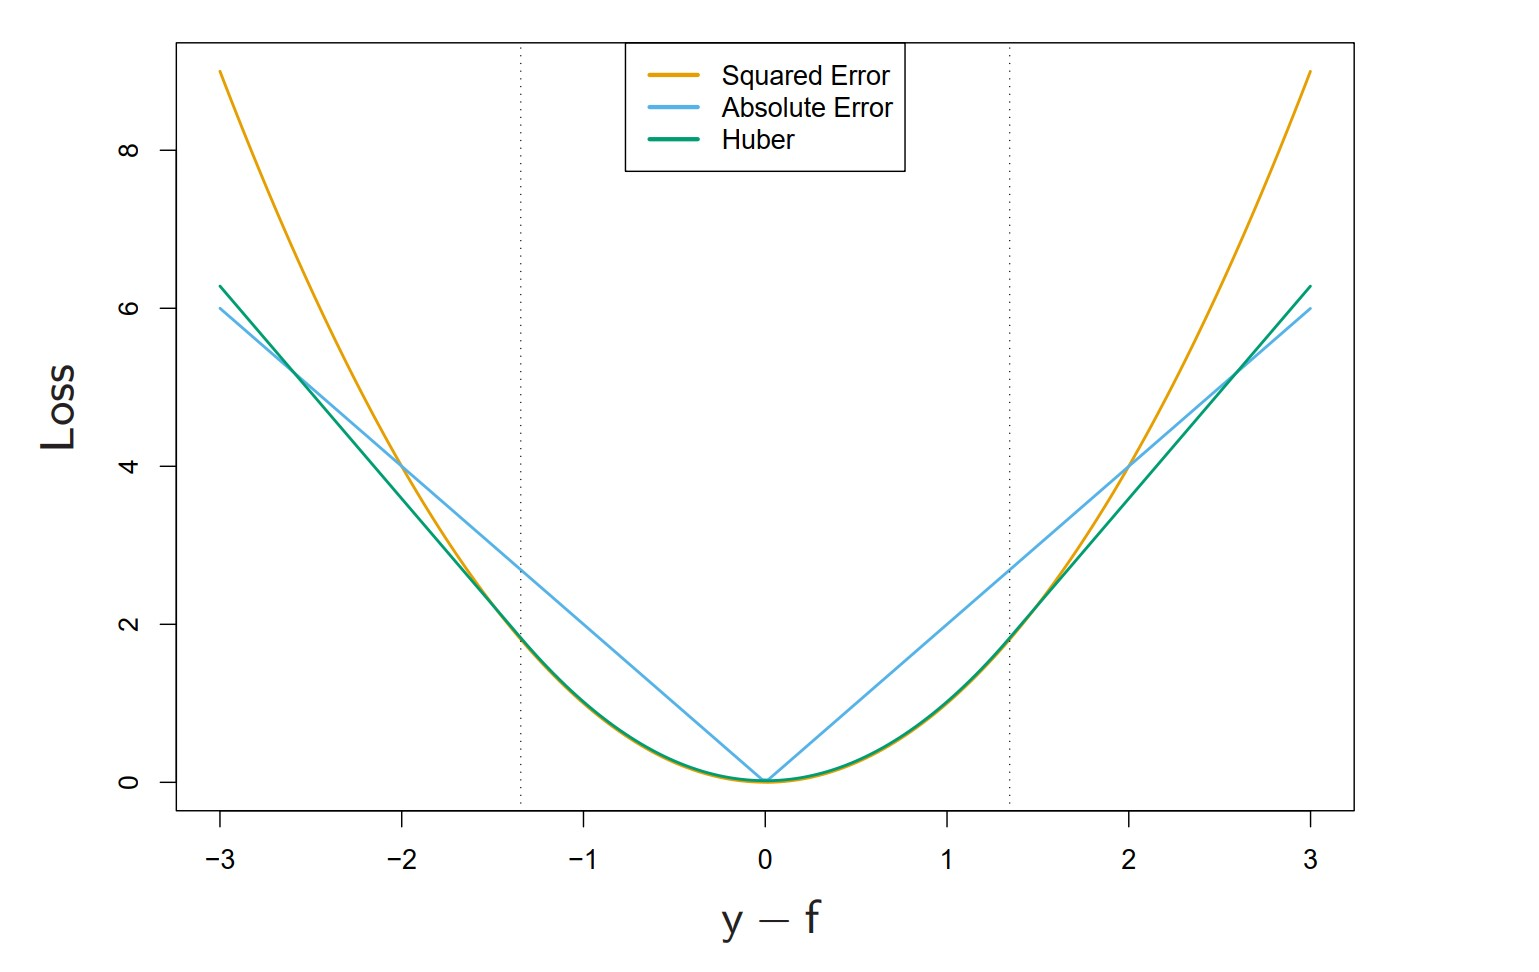
\includegraphics[width=0.6\textwidth]{regression_loss.jpg}
  \caption{平方损失函数 / 绝对值损失函数 / Huber损失函数 对比 \label{fig:regression_loss}}
\end{figure}

\begin{exercise}\label{exer:binary_loss}
  是否能够将线性回归用于二分类任务?即假定二分类任务的label为${+1,-1}$,利用Linear Regression去拟合样本点label。  
\end{exercise}
\begin{solution}
  做法可行,往往效果也不会太差。我们由
  \begin{align}
    L(f, y) &= (f-y)^2 \\
            &= (yf - 1)^2
  \end{align}
  可以看出,当margin $yf$过大时,损失函数的值也会很大。但实际如果margin是一个较大的正值,恰恰说明模型能够以高置信度将样本判为正确的label。也就是说,这样的损失函数限制了模型的学习能力(限制了一部分本可以很好完成当前二分类任务的hypothesis)。
\end{solution}



\section{分类问题的损失函数}

\subsection{二分类问题的损失函数}

最符合人类思维的二分类损失函数即为0-1 loss:
\begin{equation}
  L(\hat{y}, y) = \mathds{1}\left[\hat{y} \neq y\right]
\end{equation}

\subsection{多分类问题的损失函数}
